\documentclass{article}
\usepackage[utf8]{inputenc}
\usepackage{amsmath}
\usepackage{amssymb}
\usepackage{amsthm}
\usepackage{dsfont}
\usepackage{graphicx}
\DeclareMathOperator*{\argmin}{argmin}
\theoremstyle{definition}
\newtheorem{defi}{Définition}
\newtheorem{prop}{Propriété}
\newtheorem{theo}{Théorème}
\newtheorem{preuve}{Preuve}

\title{Analyse du dénombrements et de la présence ou absence d'espèces individuelles}
\author{Yani Bouaffad}
\date{Novembre 2020}

\begin{document}

\maketitle

\vspace{1cm}

\section*{Introduction}

L'ensemble de données "Estuary" vise à tester l'effet de la pollution de l'eau sur l'abondance de certains invertébrés marins subtidaux en comparant des échantillons d'estuaires modifiés et vierges. Dans les deux premiers tutoriels, nous avons analysé le dénombrement total des invertébrés, que nous avons supposé être continu car le dénombrement total était important. \\
Ici, nous analyserons les dénombrements et la présence / absences d'espèces individuelles, qui nécessitent des modèles mixtes linéaires généralisés. \\
Les modèles linéaires généralisés mixtes sont une extension du modèle linéaire généralisé dans lequel le prédicteur linéaire contient des effets aléatoires en plus des effets fixes habituels. 
Un effet fixe est un paramètre qui reste constant.
les effets aléatoires sont des paramètres qui sont des variables aléatoires.
\\

Dans cet exemple, nous avons un effet fixe (Modification: modifié ou vierge) et un effet aléatoire (Estuaire). 

%%%%%%%%%%%%%%%%%%%%%%%%%%%%%%%%%%%%%%%%%%%%%%%%%%%%%%%%%%%%%%%%%%%%%%%%%%%%%%%
%%%%%%%%%%%%%%%%%%%%%%%%%%%%%%%%%%%%%%%%%%%%%%%%%%%%%%%%%%%%%%%%%%%%%%%%%%%%%%%


%%%%%%%%%%%%%%%%%%%%%%%%%%%%%%%%%%%%%%%%%%%%%%%%%%%%%%%%%%%%%%%%%%%%%%%%%%%%%%%
%%%%%%%%%%%%%%%%%%%%%%%%%%%%%%%%%%%%%%%%%%%%%%%%%%%%%%%%%%%%%%%%%%%%%%%%%%%%%%%

\newpage

\section{Propriétés des modéles mixtes}

\vspace{1cm}

\subsection{Hypothèses}

Les hypothèses des modèles mixtes linéaires généralisés sont une combinaison des hypothèses des GLM et des modèles mixtes.
\\

\parindent=0em \textbf{1}. Les observés y sont indépendantsconditionnés par des prédicteurs x.\\
\textbf{2}. Les réponses proviennent d'une distribution connue de la famille exponentielle, avec une relation de variance moyenne connue.\\
\textbf{3}. Il existe une relation en ligne droite entre une fonction connue (lien) de la moyenne de y et les prédicteurs x et effets aléatoires z.\\
\textbf{4}. Effets aléatoires z sont indépendants de y.\\
\textbf{5}. Effets aléatoires z sont normalement distribués.\\



\subsection{Équation mathématiques du modéle}

\vspace{2cm}

$$\mathbf{y} = \boldsymbol{X\beta} + \boldsymbol{Zu} + \boldsymbol{\varepsilon}$$

\vspace{2cm}


\parindent=0em y est un vecteur de colonne Nx1 la variable de résultat.\\
X est une matrice N×p des p variables prédictives.\\
β est un vecteur de taille p des coefficients de régression à effets fixes (les $\beta$s).\\
Z est la matrice de design N×q pour les q effets aléatoires (le complément aléatoire du X fixe).\\
u est un vecteur de taille q des effets aléatoires (le complément aléatoire du $\beta$ fixe).\\
$\epsilon$ est un vecteur colonne de taille N, des résidus, la partie de y qui n'est pas expliquée par le modèle.
\\

\newpage 


\section{Modèle de présence ou d'absence d'hydroïdes}

Pour modéliser la présence ou absence d'hydroïdes, nous créons d'abord une variable, HydroidPres, qui vaut 1 lorsque les hydroïdes sont présents et 0 sinon. (cf fichier .ipynb)
Ce reparamétrage des données va nous permettre de faire un modèle de présence ou d'abscence d'hydroïdes.

\vspace{2cm}

Le graphique suivant donne le résumé du modèle (montre la visualisation de l'estimation de l'interception et de la modification vierge).

\begin{figure}[!h]
\includegraphics[width=0.9\textwidth]{okok.png}
\caption{Graphique estimation de l'interception et de la modification vierge}
\label{exemple somme}
\end{figure}

\vspace{2cm}

Tous les 0 sont sur une ligne (en bas à gauche) et tous les 1 ceux sont sur une ligne (en haut à droite) en raison de la discrétion des données.\\

\newpage

Malheureusement, pour les données binaires, les tracés résiduels sont assez difficiles à interpréter. 
Cela nous empêche de rechercher des modèles. \\
Nous avons le même problème avec le graphique quantile normal.
Comme on peut voir ci dessous :


\begin{center}
\begin{figure}[!h]
\centerline{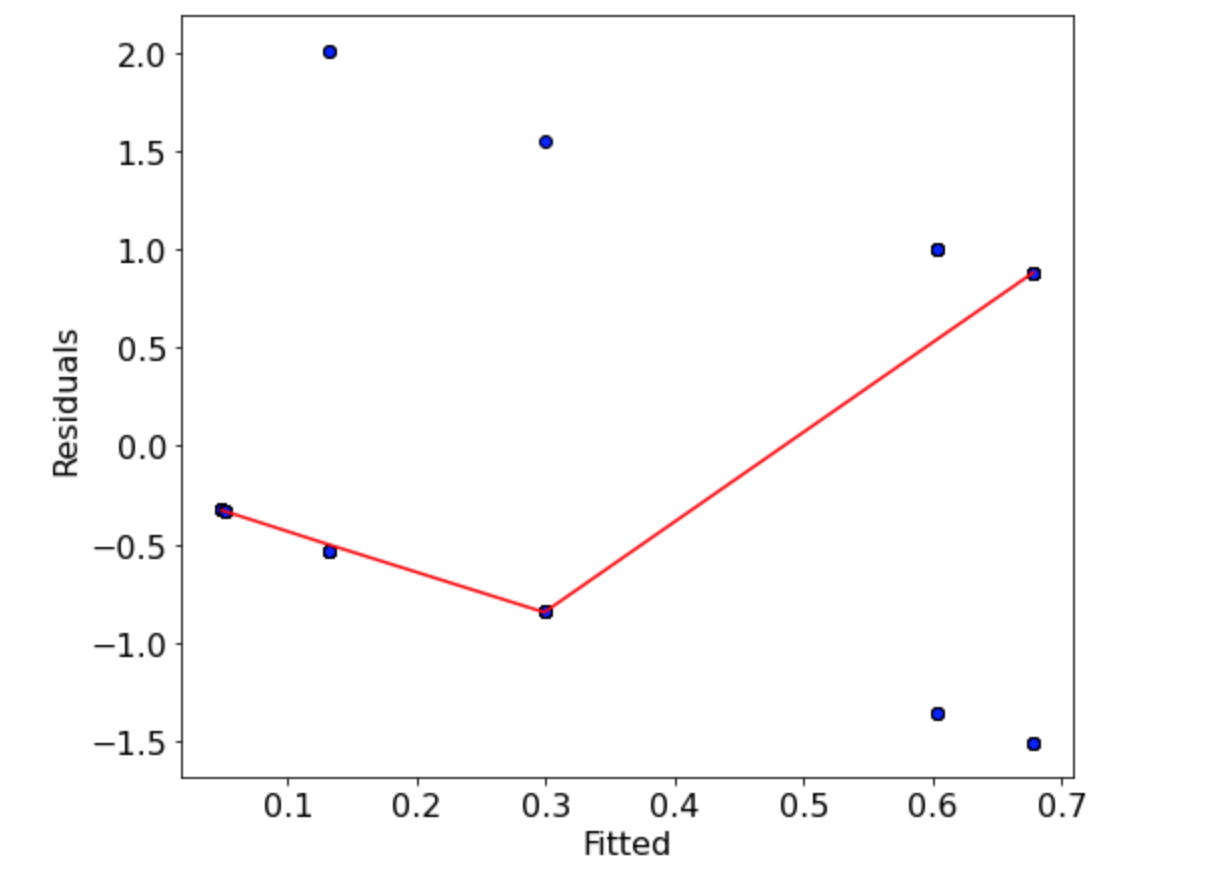
\includegraphics[width=0.6\textwidth]{bonresfit.png}}
\caption{Graphique résidus vs tracés ajustés}
\label{exemple somme}
\end{figure}


\begin{figure}[!h]
\centerline{\includegraphics[width=0.6\textwidth]{resquant.png}}
\caption{Grahique quantile normal}
\label{exemple somme}
\end{figure}
\end{center}


En examinant brièvement nos hypothèses,nous ne pouvons pas vérifier les hypothèses 1 et 4 , mais elles ne sont vraies que si nous échantillonnons au hasard.\\
Nous devrions vérifier les hypothèses 2 et 3 avec les graphiques résiduels, mais étant donné ses défauts,nous ne pouvons conclure. L'hypothèse 5 est difficile à vérifier en général mais n'est pas cruciale.



\newpage


\subsection{Test d'hypothèse}

\vspace{2cm}

\subsubsection{Bootstrap}

Pour les modèles mixtes linéaires généralisés (GLMM), nous devons utiliser le bootstrap paramétrique même pour l'inférence à effets fixes.\\
Car les valeurs p de la fonction anova sont assez approximatives pour les GLMM, même pour les effets fixes.
Parfois, la fonction lmer donnera des avertissements ou des erreurs, nous avons donc ajouté un tryCatch à ce code pour gérer cela. (cf .ipynb)


Le bootstrapping est une procédure statistique qui rééchantillonne un seul jeu de données pour créer de nombreux échantillons simulés. Ce processus vous permet de calculer les erreurs standard, de construire des intervalles de confiance et d'effectuer des tests d'hypothèse pour de nombreux types d'échantillons de statistiques. Les méthodes bootstrap sont des approches alternatives aux tests d'hypothèses traditionnels et sont remarquables pour être plus faciles à comprendre et valables pour plus de conditions.
\\
Dans notre cas nous éxécutons notre code pour 1000 échantillons bootstrap.
\\


La p-value obtenue est supérieure à la valeur seuil de 0,05 et ainsi, on ne peut pas rejeter l'hypothèse nulle, qui est qu'il n'y a pas d'effet de modification sur la présence d'hydroïdes.


\section{Modéle d'abondance}

Nous modélisons également le problème en utilisant des données de dénombrement. Les données de comptage ont une distribution de Poisson. Si les données ne correspondent pas à la relation moyenne / variance de Poisson, les choses deviennent beaucoup plus compliquées, et nous ne couvrirons pas cette situation ici dans cette étude.


Tout comme précédemment nous pouvons voir que la modification vierge est un prédicteur significatif dans ce cas également puisque la valeur p est de 0,006 donc inférieure à 0,05.


Les graphiques résiduels ne sont pas très utiles, mais nous avons au moins une idée du caractère raisonnable de l’hypothèse de variance. Il n'y a pas de forme d'éventail évidente, donc un modèle de Poisson semble correct car une forme d'éventail indiquerait une hétéroscédasticité.



\begin{figure}[!h]
\centerline{\includegraphics[width=0.6\textwidth]{resgraph.png}}
\caption{Graphique résidus vs tracés ajusté dans le cas d'un modèle poisson}
\label{exemple somme}
\end{figure}




\begin{figure}[!h]
\centerline{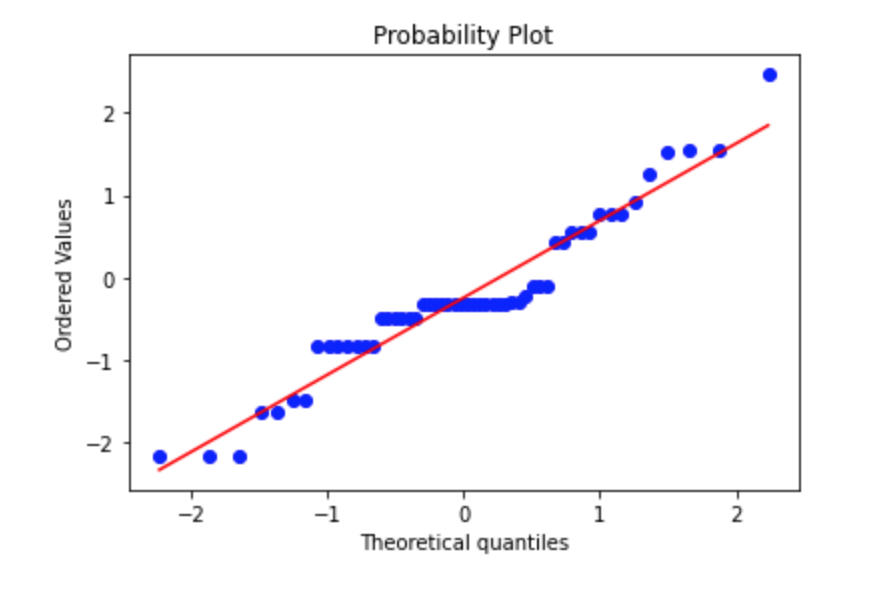
\includegraphics[width=0.6\textwidth]{eventail.png}}
\caption{Graphique quantile normal dans le cas d'un modèle poisson}
\label{exemple somme}
\end{figure}

\vspace{4cm}

\subsection{Test d'hypothèse}

On refait comme précedemment avec un bootstrap.


La valeur p obtenue est supérieure à la valeur seuil de 0,05 et donc, nous ne pouvons pas rejeter l'hypothèse nulle, à savoir qu'il n'y a pas d'effet de modification sur l'abondance des hydroïdes

\newpage

\section{Résultats}

Pour un modèle mixte simple avec un effet aléatoire, une façon dont nous pouvons rapporter les résultats est un graphique des données brutes avec les moyennes du modèle superposées. À partir du bootstrap, nous avons vu que nous ne pouvions pas rejeter l'hypothèse nulle. Il n'y a pas de preuves solides (p <0,05) d'un effet négatif de la modification sur l'abondance totale, mais nous avons pu voir que la modification est un prédicteur significatif d'hydroïde. Nous pouvons voir dans les boîtes à moustaches que la modification a des moyennes plus élevées pour JER, WAG et CLY.


\begin{figure}[!h]
\centerline{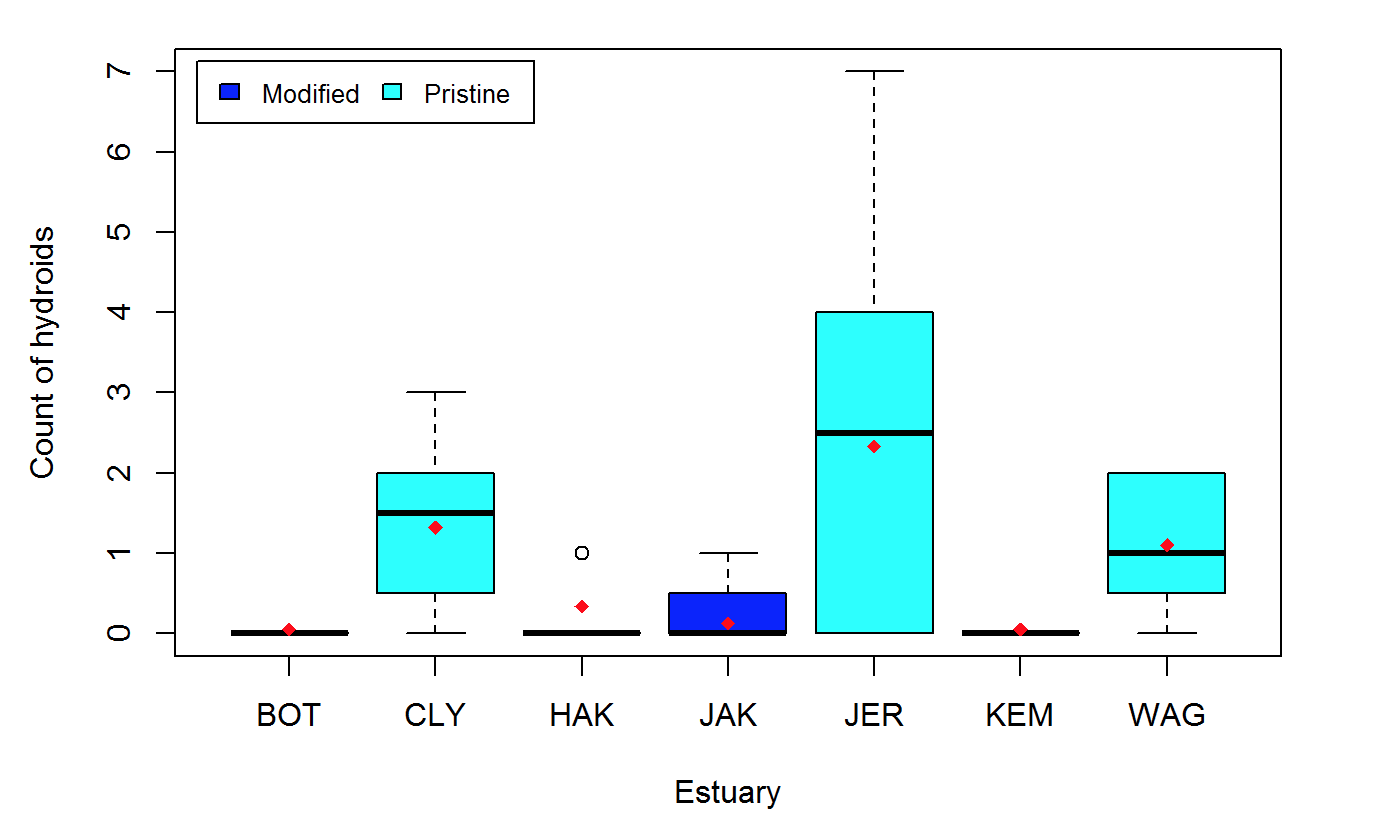
\includegraphics[width=0.6\textwidth]{boxplot.png}}
\caption{Boîtes à moustaches des modifications pour les Estuaires}
\label{exemple somme}
\end{figure}



\end{document}
